\documentclass[a4paper,11pt]{kth-mag}
\usepackage[T1]{fontenc}
\usepackage{textcomp}
\usepackage{lmodern}
\usepackage[utf8]{inputenc}
\usepackage[swedish,english]{babel}
\usepackage{modifications}
\usepackage{gnuplot-lua-tikz}

\usepackage{hyperref}
\hypersetup{colorlinks,citecolor=black,filecolor=black,linkcolor=black,urlcolor=black}

\usepackage{tikz}
\usetikzlibrary{positioning}

\usepackage{clrscode3e}
\renewcommand{\gets}{\leftarrow}

\newcommand{\AND}{}
\newcommand{\IOR}{+}
\newcommand{\XOR}{\oplus}
\newcommand{\NOT}{-}

\title{Using binary decision diagrams to determine program equivalence in a superoptimizer}
\subtitle{}
\foreigntitle{Att använda binära beslutsdiagram för att avgöra ekvivalens mellan program i en superoptimerare}
\author{Jesper Särnesjö}
\date{}
\blurb{Master's Thesis at CSC \\ Supervisor: Torbjörn Granlund \\ Examiner: Johan Håstad}
\trita{TRITA xxx yyyy-nn}

\begin{document}

\frontmatter

\pagestyle{empty}

\removepagenumbers

\maketitle

\selectlanguage{english}

\begin{abstract}
\end{abstract}

\clearpage

\begin{foreignabstract}{swedish}
\end{foreignabstract}

\clearpage

\tableofcontents*

\mainmatter

\pagestyle{newchap}

\chapter{Introduction}
\label{ch:introduction}

In the context of compiler technology, an \emph{optimizer} is a tool that attempts to improve the resource usage of programs.
Typically, an optimizer takes a program and transforms it using heuristics designed, for instance, to reduce execution time or memory usage.
Despite its name, however, an optimizer rarely makes a program \emph{optimal}.

A \emph{superoptimizer} takes a different approach.
Given a description of a function, it attempts to find, typically using some type of exhaustive search, the fastest or shortest program that computes that function.
In this way, a superoptimizer can generate programs that are indeed optimal, although with some rather strict limitations.

First, due to the inefficient nature of exhaustive search, a superoptimizer can only generate very short programs, no longer than perhaps 5 or 6 instructions, in reasonable time.
Second, a superoptimizer can only generate \emph{straight-line} programs, that is, programs that contain no loops, branches or other jumps.

Despite this, superoptimizers can be useful for optimizing inner loops and other small sequences of code required to be fast or small.

A crucial capability of a superoptimizers, is the ability to determine if a found program and the input function are \emph{equivalent}, meaning that they always yield identical output given identical and valid input.
This thesis explores using \emph{binary decision diagrams} (BDDs), data structures capable of efficiently representing Boolean functions, for this purpose.

% overview of thesis

Chapter~\ref{ch:background}

Chapter~\ref{ch:architecture}

Chapter~\ref{ch:operation}

\chapter{Background}
\label{ch:background}

\section{Superoptimizers}

\subsection{Massalin's superoptimizer}

The term \emph{superoptimizer} was coined by Massalin in a 1987 paper \cite{massalin87}, to describe a tool for finding the shortest straight-line program that computes a given function.

Massalin's implementation takes as its input a program written in assembly language for the Motorola 68020 processor.
It then consults a table containing a subset of the processor's instruction set, and begins generating all combinations of these instructions, beginning with those of length 1, then 2, and so on.
Each generated program is tested for equivalence with the input program.
When a program passes the test, it is printed, and the search terminates.
Because programs are tested in order of increasing length, this program will necessarily be \emph{optimal} in terms of length, meaning that no shorter equivalent program exists.

Naturally, exhaustively searching the space of all possible programs is a very inefficient process, considering that the number of programs of length $n$ is $b^n$, where $b$ is the \emph{branching factor} of the search tree.
To find a value of $b$, consider an architecture with $r$ registers, and an instruction set consisting of $i_0$ instructions that take no arguments, $i_1$ instructions that take one argument, and $i_2$ instructions that take two arguments.
For this architecture, the branching factor would be, in the worst case, $i_0+i_1r+i_2r^2$.
Even for modest values of $i_0$, $i_1$, $i_2$ and $r$, the branching factor would end up in the hundreds or thousands.
Hence, a naive superoptimizer is only capable of generating very short programs in reasonable time.

To address this, Massalin describes a method of \emph{pruning} the search tree.
Using this method, the superoptimizer keeps a lookup table, where short instruction sequences known to be non-optimal are marked as such.
When a program is found to contain a non-optimal instruction sequence, it is rejected without being tested.

Massalin also describes two methods of determining whether a candidate program is equivalent to the input program.

The first method, referred to as the \emph{Boolean test}, is to express both programs in Boolean logic, reduce them to an unspecified canonical form, and compare them minterm for minterm.
Using this method, Massalin's superoptimizer is capable of testing 40 programs of an unspecified length per second, when running on a 16 MHz processor.

The second method, referred to as the \emph{probabilistic test}, is to simply execute both programs with identical input, and compare their output.
This method is significantly faster, allowing the superoptimizer to test 50000 programs per second.
However, it introduces the risk of false positives, in the form of programs that are equivalent only on the input used, not in the general case.
Hence, manual verification of the output is required.
Further, whereas the Boolean test can be used on any kind of program, Massalin's probabilistic test can only be used on programs written in the assembly language of the host architecture.

It is worth noting, that even with such a significant increase in speed, only slightly longer programs may be generated in reasonable time with a realistic branching factor, as illustrated by Figure~\ref{fig:so_program_length}.

% stress this

\begin{figure}
\centering
\include{so_program_length}
\caption{The maximum length of a program generated in 24 hours, as a function of the branching factor.
The solid and dashed lines represent Massalin's superoptimizer using the Boolean and probabilistic tests, respectively.}
\label{fig:so_program_length}
\end{figure}

\subsection{GSO}

GSO, the GNU superoptimizer, is described in a 1992 paper by Granlund and Kenner \cite{granlund92}.

Like Massalin's superoptimizer, GSO optimizes for program length.
It uses a probabilistic equivalence test, and as such its output must be manually verified.
Unlike the probabilistic test in Massalin's superoptimizer, which executes instructions directly on the host architecture, GSO's test \emph{simulates} them using functions that operate on a virtual machine of sorts, consisting of a set of registers and a single carry bit.
GSO is therefore capable of supporting a wide range of architectures, but also requires that the input program be specified as a compiled-in \emph{goal function}.

Granlund and Kenner also describe numerous methods of pruning used in GSO.
When selecting arguments for generated instructions, GSO only considers live registers, that is, registers that contain input values or have previously been written to.
Similarly, instructions that read the carry flag are only generated after it has been set.
For commutative instructions, that is, instructions for which arguments can be ordered in different ways without changing the meaning of the instruction, only one argument ordering is tried.

When generating the last instruction in a program, GSO is even more restrictive.
Specifically, it requires that the last instruction reads a register or the carry flag written to by the preceding instruction, since that instruction would otherwise be superfluous.

\subsection{Denali}

Denali is a superoptimizer created by Joshi et al, then at Compaq Systems Research Center, first described in a 2002 paper \cite{joshi02}.

Denali's design differs greatly from that of Massalin's superoptimizer and GSO.
Rather than generating programs and then testing them, Denali starts by generating a set of programs equivalent to the input program, and then selects the optimal among them.

To accomplish the first step, Denali requires a set of \emph{axioms}, which describe how instructions may be substituted for another without changing the meaning of the program.
Such axioms may, for example, state that multiplication by $2^n$ is the same as right-shift by $n$.
Axioms are also used to mark instructions as commutative or associative, and to specify their identity, for instance 0 for addition and 1 for multiplication.

To select the optimal program, Denali rewrites the problem as a satisfiability problem, which is handed off to an external SAT solver.

The authors claim that Denali is capable of optimizing for \emph{execution time}, that is, the number of cycles required for the program to terminate.
This is remarkable, as determining the execution time for a program is more complicated than it may seem.
The number of cycles required to execute an instruction, depends not only on the instruction itself, but also possibly on the instructions surrounding it, due to pipelining.
In a follow-up paper \cite{joshi06}, the authors describe a simplified design, named Denali-2, which instead optimizes for program length.

% input in somewhat C-like DSL
% multiple assignments
% Alpha EV-6

\subsection{Bansal's superoptimizer}

The superoptimizer created by Bansal and described in his 2008 PhD thesis \cite{bansal_thesis} differs from the ones described above, in that it requires no human supervision, neither for verifying its output, nor for selecting its input.
Instead, it reads binaries compiled for the x86 architecture, harvesting instruction sequences to optimize.
Its output is not an optimized program, but rather the optimizations discovered.
In this way, Bansal's superoptimizer is capable of autonomously generating a very large library of optimizations, which can then be used by an ordinary peephole optimizer.

Since output is required to be correct, optimizations are verified by a Boolean test performed by a SAT solver.
To improve speed, candidate optimizations are first screened by a probabilistic test similar to that found in Massalin's superoptimizer and GSO.

% no numbers given?

Other notable features of Bansal's superoptimizer is that it is capable of optimizing both for execution time and for program size, and that it utilizes a meet-in-the-middle method of pruning.
Using this method, the superoptimizer searches not only \emph{forwards} for progressively longer programs, but also \emph{backwards} from the state the architecture is required to be in following correct program execution.

\subsection{TOAST}

TOAST, short for \emph{total optimisation using answer set technology}, is a superoptimizer created by Crick and described in his 2009 PhD thesis \cite{crick_thesis}.
It is implemented using Answer Set Programming, a declarative logic programming language.
Like Denali and Bansal's superoptimizer, it produces provably correct output.

%\subsection{...}
%
%\cite{aha}
%\cite{pic}

\section{Binary decision diagrams}

\emph{Binary decision diagrams} (BDDs) are data structures used to represent Boolean functions.
They consist of nodes, representing the function's variables. Each node has one or more incoming paths, and exactly two outgoing paths, commonly referred to as the \emph{high} and \emph{low} path.
When using a BDD to determine the value of a Boolean function, one follows a node's high path if its variable is 1, and its low path if its variable is 0, starting at the root node, until one arrives at a terminal node.

There are many types of BDDs, of which some can be used to store and manipulate Boolean functions very efficiently.
However, the performance of the operations performed on a BDD, varies greatly depending on the function represented, and the order in which its variables are indexed.

BDDs were introduced by Lee \cite{lee59}, under the name \emph{binary-decision programs}.
They were given their current name by Akers \cite{akers78}, who also explored the ideas of \emph{reducing} BDDs by removing redundant nodes, and of representing multiple functions in a single BDD.

A more restricted type of BDD was introduced by Bryant \cite{bryant86}.
In addition to the above, Bryant required the BDD to be \emph{ordered}, having its variables appear in the same order on all paths from the root to a terminal node,
and to be \emph{reduced}, containing no node with the same high and low path, and no two distinct nodes with isomorphic subgraphs.
Such a BDD is called a \emph{reduced ordered BDD} (ROBDD), and has several beneficial characteristics.
First, the algorithms used to perform Boolean operations on one or a pair of ROBDDs, are efficient, requiring at worst a number of time steps proportional to the product of the number of nodes in the two ROBDDs.
Further, ROBDDs are \emph{canonical} representations of their Boolean functions, meaning that two Boolean functions are equivalent iff their ROBDDs are isomorphic.

Bryant also further explored the idea of representing multiple functions in a single BDD, which would later be referred to as a \emph{shared BDD} by Minato et al \cite{minato90}.

A BDD with all these characteristics, a \emph{shared reduced ordered BDD} (SROBDD), has the added benefits of being memory efficient, and of allowing an isomorphism test to be implemented as a single pointer comparison.

Bryant showed that the variable ordering used can have a dramatic effect on the number of nodes in a BDD, which in the best case is linear in the number of variables, and in the worst case exponential.
Bryant states that finding the variable ordering that minimizes the number of nodes is an NP-complete problem.
Bollig and Wegener \cite{bollig96} would later show that even determining whether an ordering exists for which the number of nodes is at most a given value, is an NP-complete problem.

Bryant asserts that for many functions, a good variable ordering can be determined by examining the structure of the functions.
As an example, he mentions that for functions in which variables primarily interact pairwise, ordering variables and their partners consecutively gives good results.

However, Bryant also states that there are functions that can only be represented using a number of nodes exponential in the number of variables, regardless of variable ordering, and proves that integer multiplication is such a function.

% lower bounds given by Bollig and Wegener

\subsection{Example}

To illustrate how a moderately complex Boolean function can be represented by a BDD, consider an adder that takes two $n$-bit numbers, $a$ and $b$, and produces their sum, as well a carry-out bit.

To express the adder in Boolean logic, we represent $a$ as $n$ Boolean variables $\langle a_0, a_1, ..., a_{n-1} \rangle$, where $a_0$ and $a_{n-1}$ are the least and most significant bits of $a$, respectively.
Doing the same for $b$, we get a total of $2n$ variables.

The function for the carry-out bit, $c_{n-1}$, depends on every variable, and can be defined recursively as follows:

$$
  c_k = \left\{
  \begin{array}{ll}
    a_k \AND b_k                                             & k = 0 \\
    a_k \AND b_k \IOR a_k \AND c_{k-1} \IOR b_k \AND c_{k-1} & 0 < k < n \\
  \end{array}\right.
$$

For $n = 2$, $c_1$ can be represented as the truth table shown in Table~\ref{tab:tt_c1}, or, using the variable ordering $a_0,b_0,...,a_{n-1},b_{n-1}$, as an OBDD or ROBDD as shown in Figure~\ref{fig:bdd_c1}.
Note that the ROBDD representation is quite compact, and that not all variables are present on every path.
For instance, if $a_0$ is 0, there is no need to check $b_0$, and we instead skip ahead to $a_1$.

Not all variable orderings produce such compact ROBDDs for this function, however.
If we instead use the variable ordering $a_0,...,a_{n-1},b_0,...,b_{n-1}$, we end up with a larger ROBDD.
This becomes more clear for larger values of $n$, as illustrated in Figure~\ref{fig:bdd_c2_bad}.

Upon inspection, we find that in the ROBDD representation of this particular function, using these two variable orderings, the number of nodes is:

$$
  |c_{n-1}| = \left\{
  \begin{array}{ll}
    3n-1      & \textrm{using variable order $a_0,b_0,...,a_{n-1},b_{n-1}$} \\
    2^{n+1}-2 & \textrm{using variable order $a_0,...,a_{n-1},b_0,...,b_{n-1}$} \\
  \end{array}\right.
$$

For $n = 32$, the ROBDD would consequently contain only 97 nodes with the first variable ordering, but over 8 billion with the second.

Note that Bryant's suggested method of ordering interacting variables consecutively, works very well in this case.

\begin{table}
\centering
\begin{tabular}{cccc|cc}
$a_0$ & $b_0$ & $a_1$ & $b_1$ & $c_0$ & $c_1$ \\
\hline
0     & 0     & 0     & 0     & 0     & 0 \\
0     & 0     & 0     & 1     & 0     & 0 \\
0     & 0     & 1     & 0     & 0     & 0 \\
0     & 0     & 1     & 1     & 0     & 1 \\
0     & 1     & 0     & 0     & 0     & 0 \\
0     & 1     & 0     & 1     & 0     & 0 \\
0     & 1     & 1     & 0     & 0     & 0 \\
0     & 1     & 1     & 1     & 0     & 1 \\
1     & 0     & 0     & 0     & 0     & 0 \\
1     & 0     & 0     & 1     & 0     & 0 \\
1     & 0     & 1     & 0     & 0     & 0 \\
1     & 0     & 1     & 1     & 0     & 1 \\
1     & 1     & 0     & 0     & 1     & 0 \\
1     & 1     & 0     & 1     & 1     & 1 \\
1     & 1     & 1     & 0     & 1     & 1 \\
1     & 1     & 1     & 1     & 1     & 1 \\
\end{tabular}
\caption{Truth table for the Boolean function $c_1$.}
\label{tab:tt_c1}
\end{table}

\begin{figure}[p]
\centering
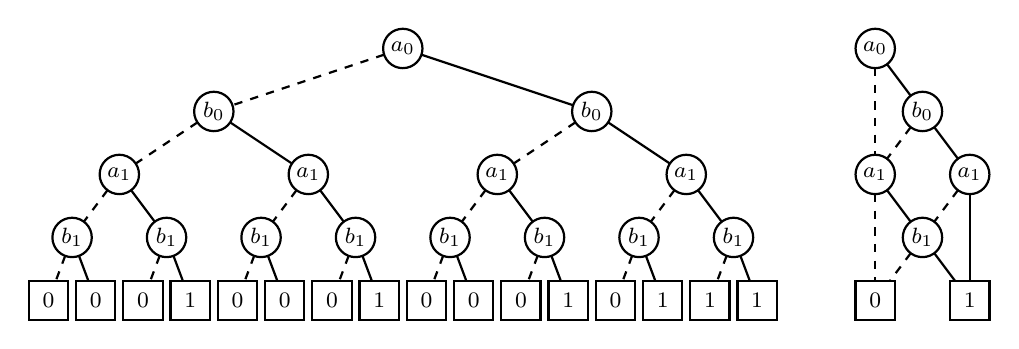
\begin{tikzpicture}
[every node/.style={draw=black,thick,minimum size=5mm,inner sep=0mm,outer sep=0mm,font=\footnotesize},
 var/.style={circle},
 val/.style={rectangle},
 thick]
\node[var] (a0)                                            {$a_0$};
\node[var] (b0A) [on grid,below  left=8mm and 24mm of a0]  {$b_0$};
\node[var] (b0B) [on grid,below right=8mm and 24mm of a0]  {$b_0$};
\node[var] (a1A) [on grid,below  left=8mm and 12mm of b0A] {$a_1$};
\node[var] (a1B) [on grid,below right=8mm and 12mm of b0A] {$a_1$};
\node[var] (a1C) [on grid,below  left=8mm and 12mm of b0B] {$a_1$};
\node[var] (a1D) [on grid,below right=8mm and 12mm of b0B] {$a_1$};
\node[var] (b1A) [on grid,below  left=8mm and  6mm of a1A] {$b_1$};
\node[var] (b1B) [on grid,below right=8mm and  6mm of a1A] {$b_1$};
\node[var] (b1C) [on grid,below  left=8mm and  6mm of a1B] {$b_1$};
\node[var] (b1D) [on grid,below right=8mm and  6mm of a1B] {$b_1$};
\node[var] (b1E) [on grid,below  left=8mm and  6mm of a1C] {$b_1$};
\node[var] (b1F) [on grid,below right=8mm and  6mm of a1C] {$b_1$};
\node[var] (b1G) [on grid,below  left=8mm and  6mm of a1D] {$b_1$};
\node[var] (b1H) [on grid,below right=8mm and  6mm of a1D] {$b_1$};
\node[val] (tA)  [on grid,below  left=8mm and  3mm of b1A] {0};
\node[val] (tB)  [on grid,below right=8mm and  3mm of b1A] {0};
\node[val] (tC)  [on grid,below  left=8mm and  3mm of b1B] {0};
\node[val] (tD)  [on grid,below right=8mm and  3mm of b1B] {1};
\node[val] (tE)  [on grid,below  left=8mm and  3mm of b1C] {0};
\node[val] (tF)  [on grid,below right=8mm and  3mm of b1C] {0};
\node[val] (tG)  [on grid,below  left=8mm and  3mm of b1D] {0};
\node[val] (tH)  [on grid,below right=8mm and  3mm of b1D] {1};
\node[val] (tI)  [on grid,below  left=8mm and  3mm of b1E] {0};
\node[val] (tJ)  [on grid,below right=8mm and  3mm of b1E] {0};
\node[val] (tK)  [on grid,below  left=8mm and  3mm of b1F] {0};
\node[val] (tL)  [on grid,below right=8mm and  3mm of b1F] {1};
\node[val] (tM)  [on grid,below  left=8mm and  3mm of b1G] {0};
\node[val] (tN)  [on grid,below right=8mm and  3mm of b1G] {1};
\node[val] (tO)  [on grid,below  left=8mm and  3mm of b1H] {1};
\node[val] (tP)  [on grid,below right=8mm and  3mm of b1H] {1};
\path[dashed] (a0)  edge (b0A);
\path         (a0)  edge (b0B);
\path[dashed] (b0A) edge (a1A);
\path         (b0A) edge (a1B);
\path[dashed] (b0B) edge (a1C);
\path         (b0B) edge (a1D);
\path[dashed] (a1A) edge (b1A);
\path         (a1A) edge (b1B);
\path[dashed] (a1B) edge (b1C);
\path         (a1B) edge (b1D);
\path[dashed] (a1C) edge (b1E);
\path         (a1C) edge (b1F);
\path[dashed] (a1D) edge (b1G);
\path         (a1D) edge (b1H);
\path[dashed] (b1A) edge (tA);
\path         (b1A) edge (tB);
\path[dashed] (b1B) edge (tC);
\path         (b1B) edge (tD);
\path[dashed] (b1C) edge (tE);
\path         (b1C) edge (tF);
\path[dashed] (b1D) edge (tG);
\path         (b1D) edge (tH);
\path[dashed] (b1E) edge (tI);
\path         (b1E) edge (tJ);
\path[dashed] (b1F) edge (tK);
\path         (b1F) edge (tL);
\path[dashed] (b1G) edge (tM);
\path         (b1G) edge (tN);
\path[dashed] (b1H) edge (tO);
\path         (b1H) edge (tP);
\node[var] (Ra0)  [on grid,right=60 mm of a0]               {$a_0$};
\node[var] (Rb0)  [on grid,below right=8mm and 6mm of Ra0]  {$b_0$};
\node[var] (Ra1A) [on grid,below  left=8mm and 6mm of Rb0]  {$a_1$};
\node[var] (Ra1B) [on grid,below right=8mm and 6mm of Rb0]  {$a_1$};
\node[var] (Rb1)  [on grid,below right=8mm and 6mm of Ra1A] {$b_1$};
\node[val] (R0)   [on grid,below  left=8mm and 6mm of Rb1]  {0};
\node[val] (R1)   [on grid,below right=8mm and 6mm of Rb1]  {1};
\path[dashed] (Ra0)  edge (Ra1A);
\path         (Ra0)  edge (Rb0);
\path[dashed] (Rb0)  edge (Ra1A);
\path         (Rb0)  edge (Ra1B);
\path[dashed] (Ra1A) edge (R0);
\path         (Ra1A) edge (Rb1);
\path[dashed] (Ra1B) edge (Rb1);
\path         (Ra1B) edge (R1);
\path[dashed] (Rb1)  edge (R0);
\path         (Rb1)  edge (R1);
\end{tikzpicture}

\caption{The Boolean function $c_1$ as an OBDD (left) and an ROBDD (right). The solid lines represent high paths and the dashed lines represent low paths.}
\label{fig:bdd_c1}
\end{figure}

\begin{figure}[p]
\centering
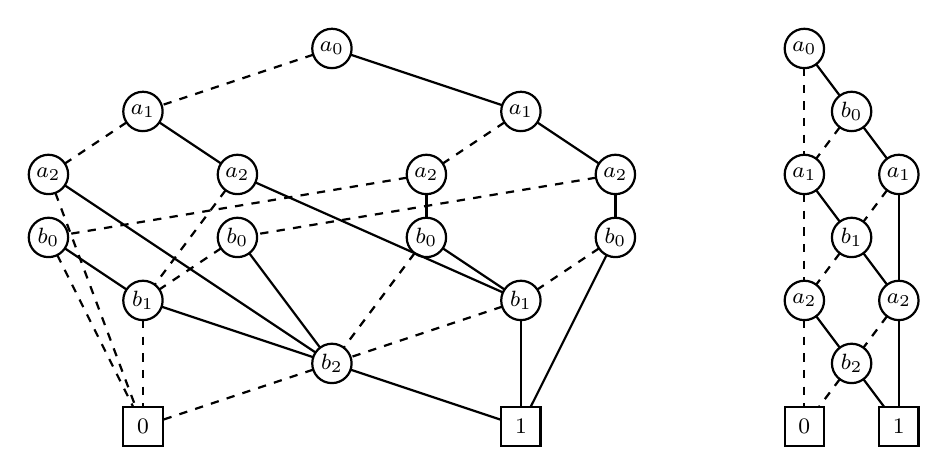
\begin{tikzpicture}
[every node/.style={draw=black,thick,minimum size=5mm,inner sep=0mm,outer sep=0mm,font=\footnotesize},
 var/.style={circle},
 val/.style={rectangle},
 thick]
\node[var] (a0)                                            {$a_0$};
\node[var] (a1A) [on grid,below  left=8mm and 24mm of a0]  {$a_1$};
\node[var] (a1B) [on grid,below right=8mm and 24mm of a0]  {$a_1$};
\node[var] (a2A) [on grid,below  left=8mm and 12mm of a1A] {$a_2$};
\node[var] (a2B) [on grid,below right=8mm and 12mm of a1A] {$a_2$};
\node[var] (a2C) [on grid,below  left=8mm and 12mm of a1B] {$a_2$};
\node[var] (a2D) [on grid,below right=8mm and 12mm of a1B] {$a_2$};
\node[var] (b0A) [on grid,below right=8mm and  0mm of a2A] {$b_0$};
\node[var] (b0B) [on grid,below right=8mm and  0mm of a2B] {$b_0$};
\node[var] (b0C) [on grid,below right=8mm and  0mm of a2C] {$b_0$};
\node[var] (b0D) [on grid,below right=8mm and  0mm of a2D] {$b_0$};
\node[var] (b1A) [on grid,below right=8mm and 12mm of b0A] {$b_1$};
\node[var] (b1B) [on grid,below right=8mm and 12mm of b0C] {$b_1$};
\node[var] (b2)  [on grid,below right=8mm and 24mm of b1A] {$b_2$};
\node[val] (0)   [on grid,below  left=8mm and 24mm of b2]  {0};
\node[val] (1)   [on grid,below right=8mm and 24mm of b2]  {1};
\path[dashed] (a0)  edge (a1A);
\path         (a0)  edge (a1B);
\path[dashed] (a1A) edge (a2A);
\path         (a1A) edge (a2B);
\path[dashed] (a1B) edge (a2C);
\path         (a1B) edge (a2D);
\path[dashed] (a2A) edge (0);
\path         (a2A) edge (b2);
\path[dashed] (a2B) edge (b1A);
\path         (a2B) edge (b1B);
\path[dashed] (a2C) edge (b0A);
\path         (a2C) edge (b0C);
\path[dashed] (a2D) edge (b0B);
\path         (a2D) edge (b0D);
\path[dashed] (b0A) edge (0);
\path         (b0A) edge (b1A);
\path[dashed] (b0B) edge (b1A);
\path         (b0B) edge (b2);
\path[dashed] (b0C) edge (b2);
\path         (b0C) edge (b1B);
\path[dashed] (b0D) edge (b1B);
\path         (b0D) edge (1);
\path[dashed] (b1A) edge (0);
\path         (b1A) edge (b2);
\path[dashed] (b1B) edge (b2);
\path         (b1B) edge (1);
\path[dashed] (b2)  edge (0);
\path         (b2)  edge (1);
\node[var] (Ga0)  [on grid,right=60mm of a0]                {$a_0$};
\node[var] (Gb0)  [on grid,below right=8mm and 6mm of Ga0]  {$b_0$};
\node[var] (Ga1A) [on grid,below  left=8mm and 6mm of Gb0]  {$a_1$};
\node[var] (Ga1B) [on grid,below right=8mm and 6mm of Gb0]  {$a_1$};
\node[var] (Gb1)  [on grid,below right=8mm and 6mm of Ga1A] {$b_1$};
\node[var] (Ga2A) [on grid,below  left=8mm and 6mm of Gb1]  {$a_2$};
\node[var] (Ga2B) [on grid,below right=8mm and 6mm of Gb1]  {$a_2$};
\node[var] (Gb2)  [on grid,below right=8mm and 6mm of Ga2A] {$b_2$};
\node[val] (G0)   [on grid,below  left=8mm and 6mm of Gb2]  {0};
\node[val] (G1)   [on grid,below right=8mm and 6mm of Gb2]  {1};
\path[dashed] (Ga0)  edge (Ga1A);
\path         (Ga0)  edge (Gb0);
\path[dashed] (Gb0)  edge (Ga1A);
\path         (Gb0)  edge (Ga1B);
\path[dashed] (Ga1A) edge (Ga2A);
\path         (Ga1A) edge (Gb1);
\path[dashed] (Ga1B) edge (Gb1);
\path         (Ga1B) edge (Ga2B);
\path[dashed] (Gb1)  edge (Ga2A);
\path         (Gb1)  edge (Ga2B);
\path[dashed] (Ga2A) edge (G0);
\path         (Ga2A) edge (Gb2);
\path[dashed] (Ga2B) edge (Gb2);
\path         (Ga2B) edge (G1);
\path[dashed] (Gb2)  edge (G0);
\path         (Gb2)  edge (G1);
\end{tikzpicture}

\caption{The Boolean function $c_2$ in ROBDD form using the variable order $a_0,a_1,a_2,b_0,b_1,b_2$ (left) and $a_0,b_0,a_1,b_1,a_2,b_2$ (right).}
\label{fig:bdd_c2_bad}
\end{figure}

\chapter{Architecture}
\label{ch:architecture}

The architecture of the superoptimizer's virtual machine is modeled after the x86, as described by the manuals issued by Intel Corporation \cite{intel_1,intel_2a,intel_2b}. % AMD?
The machine state consists of 8 32-bit registers and 5 flag bits.
The \emph{carry flag} (CF) and \emph{overflow flag} (OF) are ostensibly used to signify that an operation caused overflow when interpreted as unsigned and signed arithmetic, respectively, although many instructions treat them differently.
The \emph{parity flag} (PF) is set when an even number of the least significant 8 bits of the result are set.
The \emph{sign flag} (SF) is set equal to the most significant bit of the result.
The \emph{zero flag} (ZF) is set when the result contains no set bits.

\section{Language}

The superoptimizer takes as its input programs written in a small subset of the x86 assembly language, using Intel's syntax with a few modifications.
Registers are named r0--r7, rather than eax, ebx, etc.
Statements are terminated by semicolons rather than newlines.
Neither immediate values nor effective addresses are supported.

\section{Instruction set}

Table~\ref{tab:insns} shows the supported instructions, along with their arity and behavior with regards to flags.

\begin{table}
\centering
\begin{tabular}{lc|ccccc}
name & arity & CF & OF & PF & SF & ZF \\
\hline
stc  & 0     & 1  &    &    &    &    \\
clc  & 0     & 0  &    &    &    &    \\
cmc  & 0     & TM &    &    &    &    \\
mov  & 2     &    &    &    &    &    \\
cmov & 2     & T  & T  & T  & T  & T  \\
and  & 2     & 0  & 0  & M  & M  & M  \\
or   & 2     & 0  & 0  & M  & M  & M  \\
xor  & 2     & 0  & 0  & M  & M  & M  \\
not  & 1     &    &    &    &    &    \\
add  & 2     & M  & M  & M  & M  & M  \\
adc  & 2     & TM & M  & M  & M  & M  \\
sub  & 2     & M  & M  & M  & M  & M  \\
sbb  & 2     & TM & M  & M  & M  & M  \\
cmp  & 2     & M  & M  & M  & M  & M  \\
inc  & 1     &    & M  & M  & M  & M  \\
dec  & 1     &    & M  & M  & M  & M  \\
neg  & 1     & M  & M  & M  & M  & M  \\
\end{tabular}
\caption{The instruction set of the superoptimizer.
For the flags, 0 and 1 means that it is set to that value, M (modify) means that it is set according the result, and T (test) means that it is read.}
\label{tab:insns}
\end{table}

\chapter{Operation}
\label{ch:operation}

Its implementation consists of roughly 2000 lines of C and C++ code, as well as a test suite created to aid development.
Its design is inspired primarily by GSO.
Since my focus was on equivalence testing, the other aspects of the design were mostly kept simple.
It optimizes for program length.

\section{Input}

The superoptimizer analyzes the registers used in the input program.
Any register read from before written to is considered an input register.
The last register written to is marked as the output register.
Only a single output register is supported.

\section{Generator}

For pruning, the generator keeps track of the set of live registers.
Initially, this is equal to the set of input registers, and registers are added when written to.
Only registers in the live set are considered when selecting arguments for instructions.
Live flags are tracked in a similar way.

% cmov a != b
% leaf round

Instructions are modeled in three ways.

First, the superoptimizer has a lookup table that specifies which of an instruction's arguments, and which flags, are read from or written to.
This is used by the generator to update the live sets, and to avoid generating instructions that depend on flags not yet defined.

Second, the instructions' behavior is implemented in functions used in a probabilistic test.

Finally, and most importantly, the instructions' behavior is modeled as operations on BDDs, for use in the Boolean test.
For this, the software package BuDDy \cite{buddy} is used.

\section{Probabilistic model}

\section{BDD model}

The virtual machine's 8 32-bit registers are represented by $8 \times 32$ Boolean variables. % ordered r0b0,r1b0,...,r7b0,r1b0,etc
The flags are functions rather than variables.

\subsection{Flags}

The parity, sign and zero flags are defined in the same way for all instructions:

\begin{codebox}
\Procname{$\proc{pf}(a)$}
\zi $\id{pf} \gets \NOT(a_0 \XOR a_1 \XOR ... \XOR a_7)$
\end{codebox}

\begin{codebox}
\Procname{$\proc{sf}(a)$}
\zi $\id{sf} \gets a_{n-1}$
\end{codebox}

\begin{codebox}
\Procname{$\proc{zf}(a)$}
\zi $\id{zf} \gets \NOT(a_0 \IOR a_1 \IOR ... \IOR a_{n-1})$
\end{codebox}

\subsection{Flag control}

The simplest instructions supported by the superoptimizer are the flag control instructions \proc{stc}, \proc{clc} and \proc{cmc}.

\subsection{Data transfer}

The superoptimizer supports conditional and unconditional data transfer.
The \proc{mov} instruction is used for the latter, and is implemented as follows:

\begin{codebox}
\Procname{$\proc{mov}(a,b)$}
\zi \For $i \gets 0$ \To $n-1$
\zi \Do
      $a_i \gets b_i$
    \End
\end{codebox}

The \proc{cmov} instructions are used for conditional data transfer.
There are 30 \proc{cmov} instructions in the x86 instruction set, but only 16 with unique behavior.
They are all implemented as follows:

\begin{codebox}
\Procname{$\proc{cmov}(a,b)$}
\zi \For $i \gets 0$ \To $n-1$
\zi \Do
      $a_i \gets \NOT c \AND a_i \IOR c \AND b_i$
    \End
\end{codebox}

\subsection{Logic}

The supported instructions for bitwise logic are \proc{and}, \proc{or}, \proc{xor} and \proc{not}.
They are all simple, since each bit in the result depends only on the corresponding bit in the inputs.

\proc{and} is implemented as follows:

\begin{codebox}
\Procname{$\proc{and}(a,b)$}
\zi \For $i \gets 0$ \To $n-1$
\zi \Do
      $a_i \gets a_i \AND b_i$
    \End
\end{codebox}

\proc{or} and \proc{xor} are implemented similarly.

\proc{not} is implemented as follows:

\begin{codebox}
\Procname{$\proc{not}(a,b)$}
\zi \For $i \gets 0$ \To $n-1$
\zi \Do
      $a_i \gets \NOT a_i$
    \End
\end{codebox}

\subsection{Addition and subtraction}

The \proc{add}, \proc{adc}, \proc{sub}, \proc{sbb}, \proc{cmp}, \proc{inc}, \proc{dec} and \proc{neg} instructions are all variants of addition.

\proc{add} is implemented as follows:

\begin{codebox}
\Procname{$\proc{add}(a,b)$}
\zi $c_0 \gets a_0 \AND b_0$
\zi $a_0 \gets a_0 \XOR b_0$
\zi \For $i \gets 1$ \To $n-1$
\zi \Do
      $c_i \gets a_i \AND b_i \IOR a_i \AND c_{i-1} \IOR b_i \AND c_{i-1}$
\zi   $a_i \gets a_i \XOR b_i \XOR c_{i-1}$
    \End
\end{codebox}

\begin{codebox}
\zi $\id{cf} \gets c_{n-1}$
\zi $\id{of} \gets c_{n-1} \XOR c_{n-2}$
\end{codebox}

For \proc{adc} and \proc{sbb}, \id{cf} is taken into account when \id{c_0} and \id{a_0} are set.
For \proc{sub} and \proc{sbb}, the two's complement of \id{b} is used.
\proc{cmp} behaves like \proc{sub}, except it does not modify \id{a}.
\proc{inc} and \proc{dec} behave like \proc{add} and \proc{sub}, with fixed values for \id{b}.

\proc{neg} behaves like \proc{inc}, with the values for \id{a} inverted.
Further, it sets the carry flag if a is non-zero:

\begin{codebox}
\zi $\id{cf} \gets a_0 + a_1 + ... + a_{n-1}$
\end{codebox}

\subsection{Multiplication}

\chapter{Results}
\label{ch:results}

\section{...}

% give example of programs that pass probabilistic test but not BDD test

\section{Performance}

\chapter{Recommendations}
\label{ch:recommendations}

\bibliographystyle{ieeetr}
\bibliography{thesis}

\end{document}
